\documentclass[11pt]{article}
\usepackage[T1]{fontenc}
\renewcommand{\rmdefault}{ptm}
\usepackage[paperwidth=297mm,paperheight=210mm,margin=0mm]{geometry}
\usepackage{amsmath,amssymb,booktabs,graphicx,tikz}
\usetikzlibrary{arrows.meta,calc}
\definecolor{ink}{HTML}{243746}
\definecolor{axa}{HTML}{D17B14}
\definecolor{axd}{HTML}{963D98}
\definecolor{axx}{HTML}{1765B0}
\definecolor{axy}{HTML}{C43C39}
\definecolor{axz}{HTML}{22854E}
\pagestyle{empty}
\begin{document}\null
\begin{tikzpicture}[remember picture,overlay,x=1mm,y=-1mm,
  originmark/.style={circle,draw=ink,fill=white,inner sep=1.3pt,line width=.65pt},
  dimlabel/.style={fill=white,inner sep=1.2pt,font=\small},
  al/.style={-{Latex[length=1.7mm]},draw=axa,line width=1.0pt},
  dl/.style={-{Latex[length=1.7mm]},draw=axd,line width=1.0pt}]
\begin{scope}[shift={(current page.north west)}]
\node[anchor=north west,text=ink,font=\bfseries\Large] at (10.000,8.000) {Head and neck: origins, D-H distances and axes};
\node[anchor=north west,text=ink,font=\small] at (10.000,20.000) {Direct annotations on the original assignment drawing. Zero pose; distances in mm.};
\draw[ink!30] (10,29)--(287,29);
\node[anchor=north west,inner sep=0pt,opacity=.70] at (4.000,41.000) {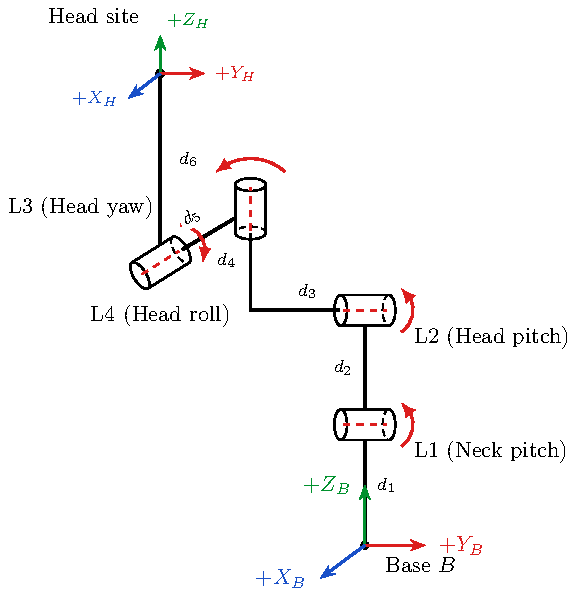
\includegraphics[width=119.540mm]{../assets/assignment_head_original.pdf}};
\draw[ink!50,densely dashed,line width=.5pt] (57.250,128.505)--(101.250,128.505);
\draw[ink!50,densely dashed,line width=.5pt] (35.600,105.070)--(90.600,105.070);
\draw[ink!50,densely dashed,line width=.5pt] (55.600,65.570)--(55.600,107.570);
\draw[ink!50,densely dashed,line width=.5pt] (21.110,103.620)--(65.110,78.020);
\draw[al] (79.250,128.505)--(79.250,105.070);
\node[dimlabel,text=axa] at (86.250,116.787) {$a_1^{\rm DH}$};
\draw[dl] (79.250,105.070)--(55.600,105.070);
\node[dimlabel,text=axd] at (67.425,111.070) {$d_2^{\rm DH}$};
\draw[dl] (55.600,105.070)--(55.600,83.570);
\node[dimlabel,text=axd] at (62.600,95.320) {$d_3^{\rm DH}$};
\draw[dl] (55.600,83.570)--(37.110,94.320);
\draw[ink!65,line width=.4pt] (46.355,88.945)--(7,88.945)--(7,145.945)--(21.355,145.945);
\node[dimlabel,text=axd] at (21.355,145.945) {$d_4^{\rm DH}$};
\draw[dl] (37.110,94.320)--(37.110,56.050);
\node[dimlabel,text=axd] at (30.110,75.185) {$d_5^{\rm DH}$};
\node[originmark] at (79.250,153.445) {};
\draw[ink!65,line width=.45pt] (79.250,153.445)--(95.250,164.445);
\node[fill=white,inner sep=1pt,text=ink,font=\small] at (95.250,164.445) {$B$};
\node[originmark] at (79.250,128.505) {};
\draw[ink!65,line width=.45pt] (79.250,128.505)--(99.250,142.505);
\node[fill=white,draw=ink!25,rounded corners=.6mm,inner sep=2pt,text=ink,font=\small] at (99.250,142.505) {\shortstack{$O_0=O_1$\\{\fontsize{7}{8}\selectfont \textcolor{axx}{$x_1=+Z$}\;\textcolor{axy}{$y_1=-X$}\;\textcolor{axz}{$z_1=-Y$}}\\{\fontsize{7}{8}\selectfont \textcolor{axx}{$x_0=+X$}\;\textcolor{axy}{$y_0=+Y$}\;\textcolor{axz}{$z_0=+Z$}}}};
\node[originmark] at (79.250,105.070) {};
\draw[ink!65,line width=.45pt] (79.250,105.070)--(96.250,95.070);
\node[fill=white,inner sep=1pt,text=ink,font=\small] at (96.250,95.070) {$P_{2}$};
\node[originmark] at (55.600,105.070) {};
\draw[ink!65,line width=.45pt] (55.600,105.070)--(54.600,127.070);
\node[fill=white,draw=ink!25,rounded corners=.6mm,inner sep=2pt,text=ink,font=\small] at (54.600,127.070) {\shortstack{$O_{2}$\\{\fontsize{7}{8}\selectfont \textcolor{axx}{$x_{2}=+X$}\;\textcolor{axy}{$y_{2}=+Z$}\;\textcolor{axz}{$z_{2}=-Y$}}}};
\node[originmark] at (55.600,83.570) {};
\draw[ink!65,line width=.45pt] (55.600,83.570)--(93.600,76.570);
\node[fill=white,draw=ink!25,rounded corners=.6mm,inner sep=2pt,text=ink,font=\small] at (93.600,76.570) {\shortstack{$O_{3}$\\{\fontsize{7}{8}\selectfont \textcolor{axx}{$x_{3}=+Y$}\;\textcolor{axy}{$y_{3}=-X$}\;\textcolor{axz}{$z_{3}=+Z$}}}};
\node[originmark] at (37.110,94.320) {};
\draw[ink!65,line width=.45pt] (37.110,94.320)--(17,94.320)--(17,117.320)--(28.110,117.320);
\node[fill=white,draw=ink!25,rounded corners=.6mm,inner sep=2pt,text=ink,font=\small] at (28.110,117.320) {\shortstack{$O_{4}$\\{\fontsize{7}{8}\selectfont \textcolor{axx}{$x_{4}=+Y$}\;\textcolor{axy}{$y_{4}=-Z$}\;\textcolor{axz}{$z_{4}=-X$}}}};
\node[originmark] at (37.110,56.050) {};
\draw[ink!65,line width=.45pt] (37.110,56.050)--(97.110,47.050);
\node[fill=white,draw=ink!25,rounded corners=.6mm,inner sep=2pt,text=ink,font=\small] at (97.110,47.050) {\shortstack{$O_{5}$ (site)\\{\fontsize{7}{8}\selectfont \textcolor{axx}{$x_{5}=+X$}\;\textcolor{axy}{$y_{5}=+Y$}\;\textcolor{axz}{$z_{5}=+Z$}}}};
\node[anchor=north west,text=ink,font=\small] at (8.000,182.000) {\textcolor{axa}{Orange: $a_{i-1}^{\rm DH}$}\quad\textcolor{axd}{Purple: $d_i^{\rm DH}$}};
\node[anchor=north west,text=ink,text width=117mm,font=\footnotesize] at (8.000,190.000) {Original black $d$ labels are handout dimensions. Coloured superscript DH labels are table parameters.};
\node[anchor=north west,text=ink,font=\normalsize] at (137.000,34.000) {\textbf{Read each row as a two-step path}};
\node[anchor=north west,text=ink,font=\normalsize] at (137.000,43.000) {$O_{i-1}\xrightarrow[+x_{i-1}]{a_{i-1}}P_i\xrightarrow[+z_i]{d_i}O_i$};
\node[anchor=north west,text=ink,font=\small] at (137.000,54.000) {A negative value means travel opposite to that positive axis.};
\node[anchor=north west,text=ink,font=\small,inner sep=0pt] at (138.000,63.000) {\begin{tabular}{c|rr|cc}
$i$ & $a_{i-1}$ & $d_i$ & axis for $a$ & axis for $d$\\\hline
$1$ & $0$ & $0$ & $+X$ & $-Y$\\
$2$ & $66$ & $19.05$ & $+Z$ & $-Y$\\
$3$ & $0$ & $37.85$ & $+X$ & $+Z$\\
$4$ & $0$ & $-5$ & $+Y$ & $-X$\\
$5$ & $0$ & $42.45$ & $+Y$ & $+Z$\\
\end{tabular}};
\node[anchor=north west,text=ink,font=\footnotesize,align=left] at (137.000,102.000) {$a_0=a_2=a_3=a_4=0$; $d_1=0$.\\$P_1=O_0=O_1$, $P_3=O_2$, $P_4=O_3$, $P_5=O_4$.};
\node[anchor=north west,text=ink,font=\normalsize] at (137.000,114.000) {\textbf{Full frame axes, expressed in base $B$}};
\node[anchor=north west,text=ink,font=\small,inner sep=0pt] at (138.000,124.000) {\begin{tabular}{c|ccc}
frame & \textcolor{axx}{$+x_i$} & \textcolor{axy}{$+y_i$} & \textcolor{axz}{$+z_i$}\\\hline
$0$ & $+X$ & $+Y$ & $+Z$\\
$1$ & $+Z$ & $-X$ & $-Y$\\
$2$ & $+X$ & $+Z$ & $-Y$\\
$3$ & $+Y$ & $-X$ & $+Z$\\
$4$ & $+Y$ & $-Z$ & $-X$\\
$5$ & $+X$ & $+Y$ & $+Z$\\
\end{tabular}};
\node[anchor=north west,text=ink,font=\footnotesize,text width=56mm,align=center] at (231.000,61.000) {\textbf{Positive-axis triads}\newline Translated from their $O_i$};
\node[text=ink,font=\small] at (244.000,75.000) {$i=0,5$};
\draw[-{Latex[length=1.4mm]},axx,line width=.8pt] (244.000,87.000)--(239.200,90.600);
\node[text=axx,font=\footnotesize,inner sep=0pt] at (237.120,92.160) {$x_i$};
\draw[-{Latex[length=1.4mm]},axy,line width=.8pt] (244.000,87.000)--(250.000,87.000);
\node[text=axy,font=\footnotesize,inner sep=0pt] at (252.600,87.000) {$y_i$};
\draw[-{Latex[length=1.4mm]},axz,line width=.8pt] (244.000,87.000)--(244.000,81.000);
\node[text=axz,font=\footnotesize,inner sep=0pt] at (244.000,78.400) {$z_i$};
\fill[ink] (244.000,87.000) circle[radius=.45mm];
\node[text=ink,font=\small] at (274.000,75.000) {$i=1$};
\draw[-{Latex[length=1.4mm]},axx,line width=.8pt] (274.000,87.000)--(274.000,81.000);
\node[text=axx,font=\footnotesize,inner sep=0pt] at (274.000,78.400) {$x_i$};
\draw[-{Latex[length=1.4mm]},axy,line width=.8pt] (274.000,87.000)--(278.800,83.400);
\node[text=axy,font=\footnotesize,inner sep=0pt] at (280.880,81.840) {$y_i$};
\draw[-{Latex[length=1.4mm]},axz,line width=.8pt] (274.000,87.000)--(268.000,87.000);
\node[text=axz,font=\footnotesize,inner sep=0pt] at (265.400,87.000) {$z_i$};
\fill[ink] (274.000,87.000) circle[radius=.45mm];
\node[text=ink,font=\small] at (244.000,104.000) {$i=2$};
\draw[-{Latex[length=1.4mm]},axx,line width=.8pt] (244.000,116.000)--(239.200,119.600);
\node[text=axx,font=\footnotesize,inner sep=0pt] at (237.120,121.160) {$x_i$};
\draw[-{Latex[length=1.4mm]},axy,line width=.8pt] (244.000,116.000)--(244.000,110.000);
\node[text=axy,font=\footnotesize,inner sep=0pt] at (244.000,107.400) {$y_i$};
\draw[-{Latex[length=1.4mm]},axz,line width=.8pt] (244.000,116.000)--(238.000,116.000);
\node[text=axz,font=\footnotesize,inner sep=0pt] at (235.400,116.000) {$z_i$};
\fill[ink] (244.000,116.000) circle[radius=.45mm];
\node[text=ink,font=\small] at (274.000,104.000) {$i=3$};
\draw[-{Latex[length=1.4mm]},axx,line width=.8pt] (274.000,116.000)--(280.000,116.000);
\node[text=axx,font=\footnotesize,inner sep=0pt] at (282.600,116.000) {$x_i$};
\draw[-{Latex[length=1.4mm]},axy,line width=.8pt] (274.000,116.000)--(278.800,112.400);
\node[text=axy,font=\footnotesize,inner sep=0pt] at (280.880,110.840) {$y_i$};
\draw[-{Latex[length=1.4mm]},axz,line width=.8pt] (274.000,116.000)--(274.000,110.000);
\node[text=axz,font=\footnotesize,inner sep=0pt] at (274.000,107.400) {$z_i$};
\fill[ink] (274.000,116.000) circle[radius=.45mm];
\node[text=ink,font=\small] at (244.000,133.000) {$i=4$};
\draw[-{Latex[length=1.4mm]},axx,line width=.8pt] (244.000,145.000)--(250.000,145.000);
\node[text=axx,font=\footnotesize,inner sep=0pt] at (252.600,145.000) {$x_i$};
\draw[-{Latex[length=1.4mm]},axy,line width=.8pt] (244.000,145.000)--(244.000,151.000);
\node[text=axy,font=\footnotesize,inner sep=0pt] at (244.000,153.600) {$y_i$};
\draw[-{Latex[length=1.4mm]},axz,line width=.8pt] (244.000,145.000)--(248.800,141.400);
\node[text=axz,font=\footnotesize,inner sep=0pt] at (250.880,139.840) {$z_i$};
\fill[ink] (244.000,145.000) circle[radius=.45mm];
\node[anchor=north west,text=ink,text width=149mm,font=\footnotesize,align=left] at (137.000,161.000) {$O_0=O_1$ at the neck axis; their orientations differ. $P_2$ is the pitch-axis point vertically above $O_1$. $O_2$ is shifted along the head-pitch axis. $O_3$ and $O_4$ lie on extended yaw and roll axes. The base-to-neck transform $^BT_0$ is separate. The handout's $d_1=92.021$ mm is not the D-H $d_1=0$.};
\node[anchor=north west,text=ink,text width=149mm,font=\footnotesize,align=left] at (137.000,192.000) {Original: Assignment 1, Fig. 4. Schematic, not to scale; perspective is illustrative. Exact signs and directions are given in the tables. Markers are selected D-H origins, not CAD joint centres.};
\end{scope}
\end{tikzpicture}
\end{document}
